Ebben a fejezetben szeretnék egy átfogó képet adni az általam létrehozott helpdesk alkalmazásról. Az egyes komponensek részletes leírása \aref{ch:implementacio}. fejezetben található.

\section{Legfontosabb komponensek}

\begin{figure}[hbt] 
	\centering
	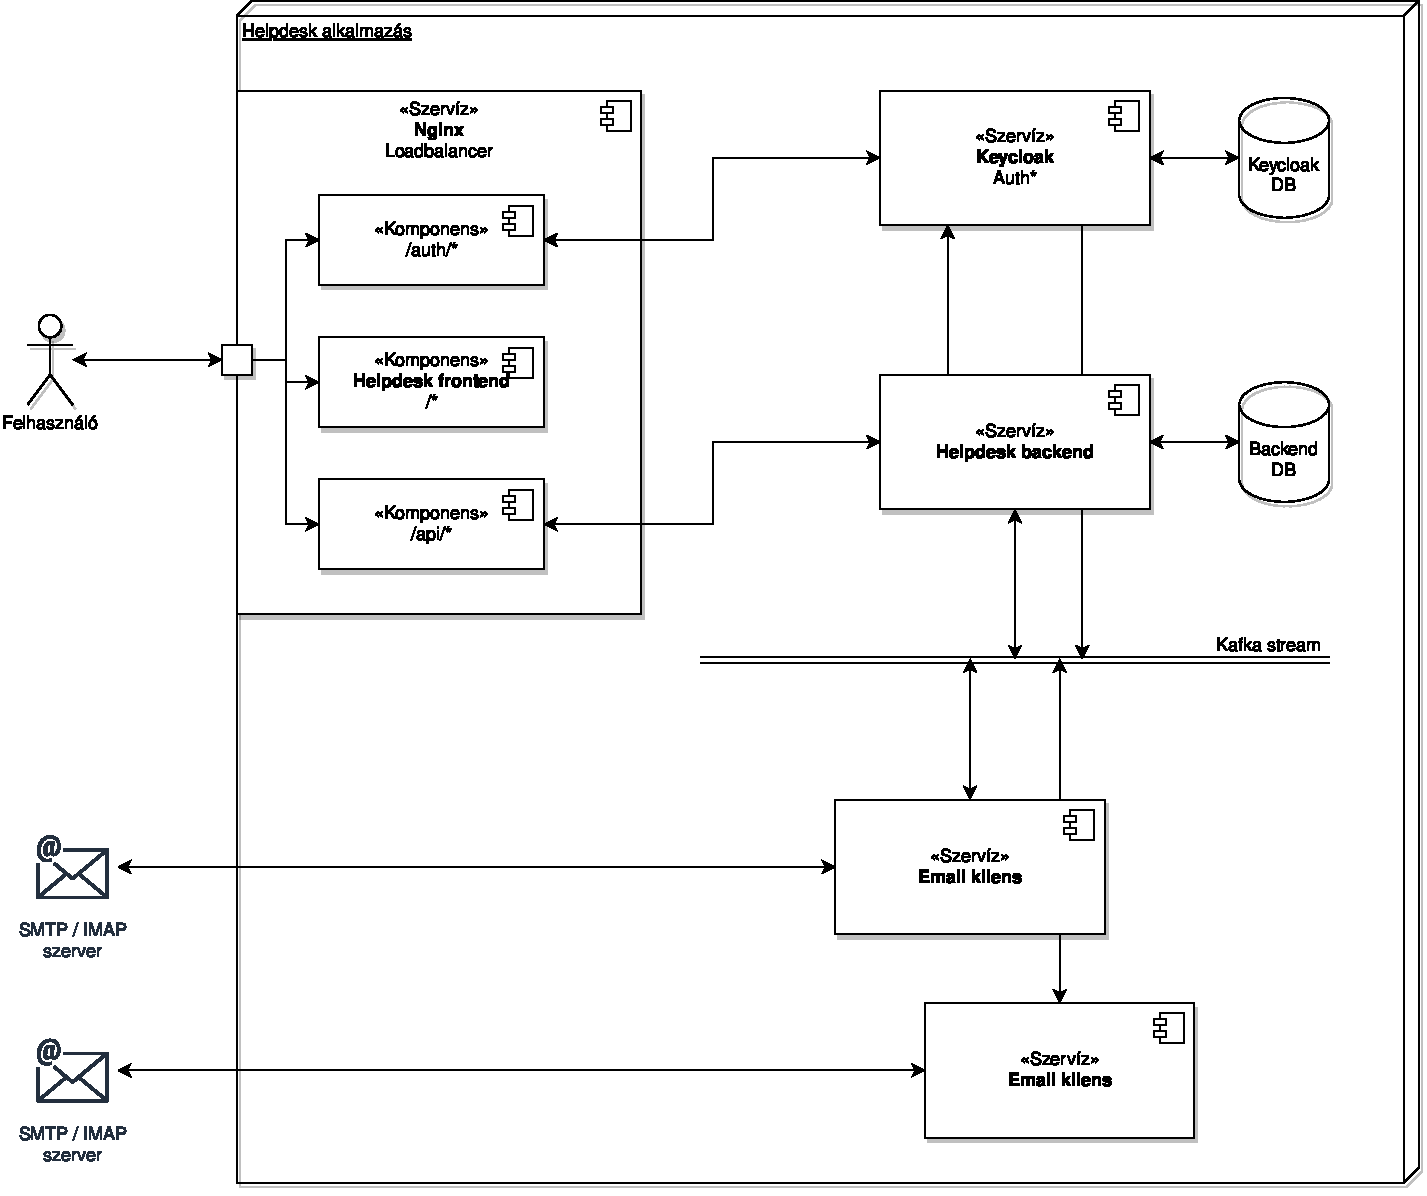
\includegraphics[width=0.87\textwidth]{komponens_diagram_drawio.pdf}
	\caption{A legfontosabb komponensek}
	\label{fig:komponens_diagram}
	\floatfoot{Forrás: saját ábra}
\end{figure}

\Aref{fig:komponens_diagram}. ábrán a legfontosabb szervizeket gyűjtöttem össze. Az üzleti funkcionalitás megvalósulása az itt bemutatott komponensek összehangolt munkáján keresztül valósul meg.



\begin{itemize}
	\item A felhasználó az nginx-en (\ref{sec:nginx} pont) keresztül éri el a heldesk alkalmazást.
	\item Az nginx dönti el, hogy melyik URL-t melyik szerviz szolgálja ki.
	\item Az email kliens és a heldpesk backend kafka streamen keresztül éri el egymást.
	\item Az email kliensek kezelik az e-mail szerverekkel való adatcserét.
\end{itemize}


\section{Adatbázis UML diagram}
A helpdesk backend adatbázis legfontosabb tábláit \aref{fig:basic_database_uml}. ábra tartalmazza. Az ábrán nem szerepelnek az audithoz, és a Liquibase által használt táblák~(\ref{sec:adatbazis} pont). \Aref{ch:bemutatas}. fejezetben található \ref{fig:extended_database_uml}. ábra tartalmazza az adatbázis összes tábláját.
 


\begin{figure}[hbt] 
	\centering
	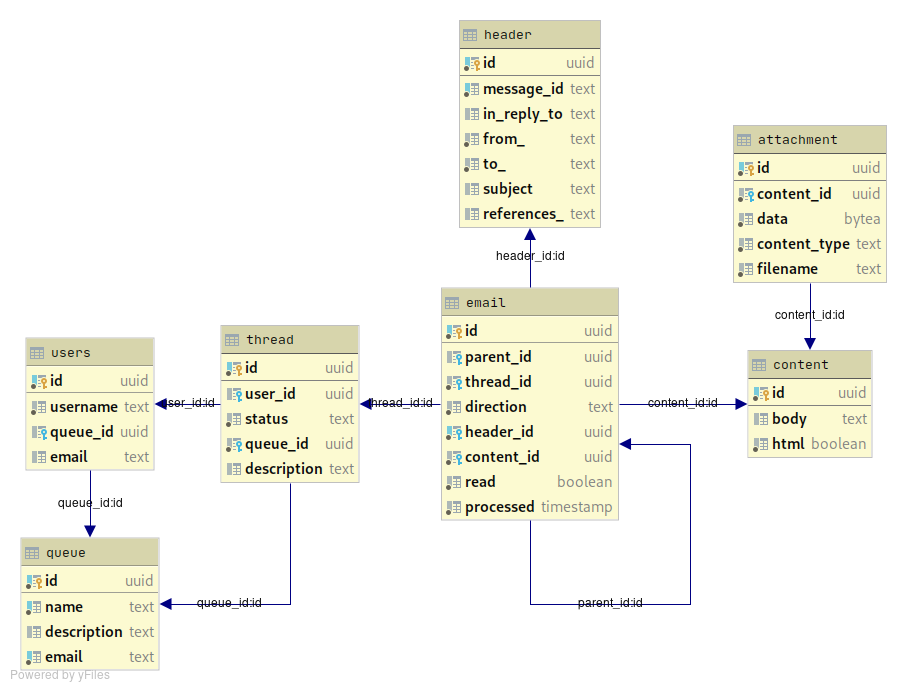
\includegraphics[width=0.85\textwidth]{basic_database_uml.png}
	\caption{A backend legfontosabb adatbázistáblái}
	\label{fig:basic_database_uml}
	\floatfoot{Forrás: saját ábra}
\end{figure}

\section{E-mail fogadásának és küldésének folyamata}
A könnyebb átláthatóság érdekében, a folyamatokat egy e-mail szemszögéből mutatom be \aref{fig:path_of_an_email}. ábrán. Az e-mail fogadása során:
\begin{enumerate}
	\item Az e-mail kliens IMAP protokollon keresztül megkapja az új e-mailt.
	\item Az e-mail kliens a bejövő e-mailt egy kafka üzenetként teszi közzé a bejövő e-mailek kafka \textit{topicban}.
	\item A bejövő e-mailek \textit{topic}ra feliratkozott helpdesk backend megkapja a kafka üzenetet.
	\item A helpdesk backend eltárolja az új üzenetet az adatbázisban
	\item A felhasználó a frontend segítségével lekérdezi az újonnan beérkezett e-maileket.
	\item A helpdesk backend a kérésre elküldi az újonnan fogadott e-mailt.
\end{enumerate}

\bigskip
Az e-mail küldése során:
\begin{enumerate}
	\item A felhasználó az új e-mail elolvasása után a frontend segítségével megírja a választ.
	\item A felhasználó elküldi a választ a helpdesk backendnek.
	\item A helpdesk backend eltárolja az adatbázisba az új e-mailt, majd az e-mail szálnak megfelelő kimenő e-mail \textit{topic}ba közzéteszi az új üzenetet.
	\item Az e-mail cím specifikus kimenő e-mailek \textit{topic}ra feliratkozott e-mail kliens megkapja a kafka üzenetet.
	\item Az e-mail kliens SMTP protokollon keresztül elküldi az új e-mailt.
\end{enumerate}


\begin{figure}[hbt] 
	\centering
	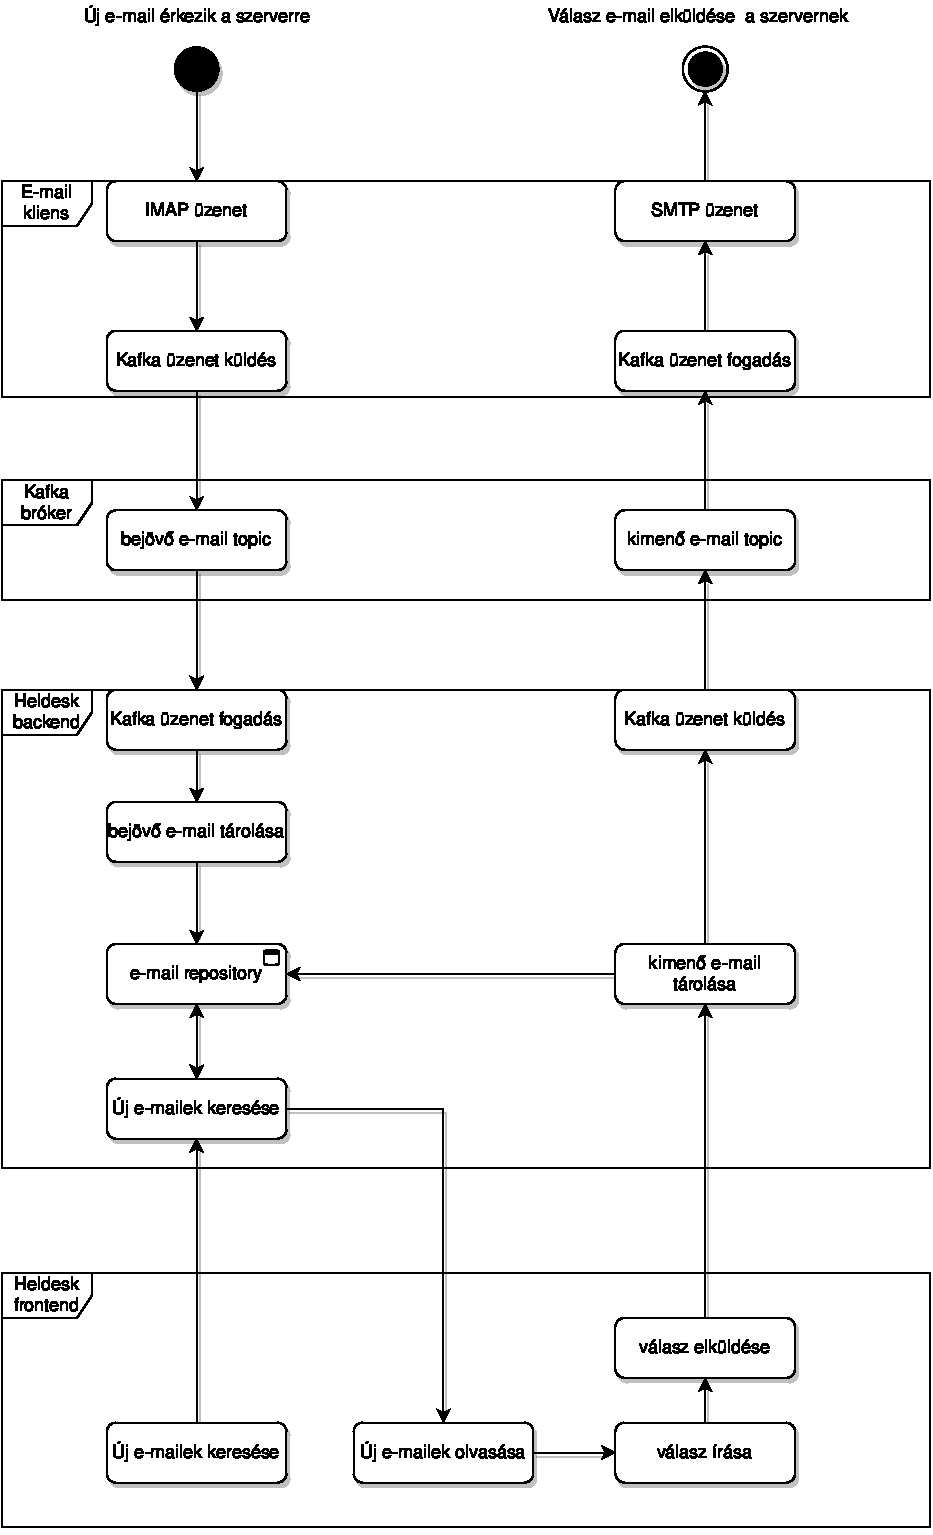
\includegraphics[width=0.7\textwidth]{path_of_an_email_drawio.pdf}
	\caption{A bejövő és kimenő e-mail útja}
	\label{fig:path_of_an_email}
	\floatfoot{Forrás: saját ábra}
\end{figure}
